\begin{figure}[h]
\caption{\\The structure of the Hidden Markov Model}
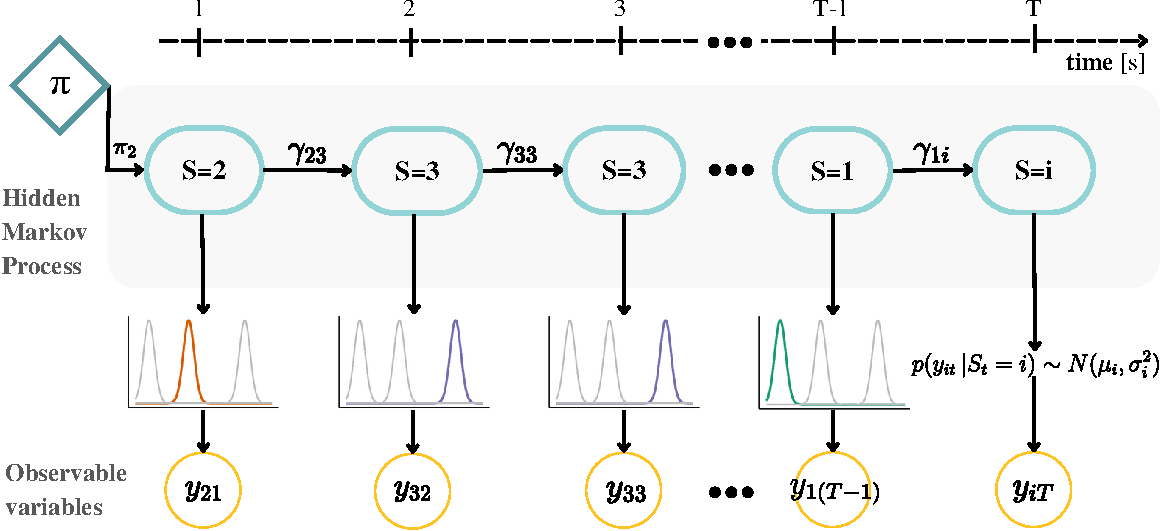
\includegraphics[width=\textwidth]{graphics/time_hmm_2.pdf}
\flushleft
\footnotesize
\justifying
The figure shows the structure of the Hidden Markov Model based on three hidden states and one normally distributed dependent variable. The model can be defined by three sets of parameters: 1) the vector $\pi$ of initial probabilities where $\pi_2$ is a probability of $S=2$ to be the initial state, 2) the TPM $\Gamma$ with $\gamma_{ij}$ for ${i,j \in \{1,2,3\}}$, and $\gamma_{23}$ represents the probability of switching from $S=2$ to $S=3$, and 3) the state-specific emission distributions of observed events $y_t$. At each point in time, the system transition to a new state, e.g., $S=3$ at $t=2$, one outcome measure $y_{32}$ is drawn from Normal emission distribution (highlighted in purple) with state-specific parameters.
 \label{hmm_fig}
\end{figure}
\section{Theoretical Background}
\subsection{Hidden Markov Model}
The Hidden Markov Model is a statistical method used to infer hidden states ${S_t \in (1,2,...,m)}$ at each time point ${t=1,.., M}$ from the observed series ${(y_1,y_t,...,y_M)}$, where $m$ is the total number of states, $y_t$ is a measurement at a given time point $t$ and $M$ is the total length of the series. The method measures the dynamics of discrete hidden states via the dynamics of the observable shifts in measurements. A detailed illustrative example of the structure of \ac{hmm} in Figure \ref{hmm_fig}. 


The \ac{hmm} is driven by two main assumptions. The first one states that all hidden states follow a Markov Process (Hidden Markov Process) meaning that the conditional probability distribution of future states depends only upon the present state at any point in time (also known as the memoryless assumption). We refer readers to Figure \ref{hmm_fig2}A where the assumption can be further inspected. In terms of probability equations, the property is defined as: 
\begin{equation}
 Pr(S_t=i \rightarrow S_{t+1}=j)=Pr(S_{t+1}=j|S_{t}=i)=\gamma_{ij}
 \label{ee1}
\end{equation}
i.e. the probability of switching from state $i$ at time point $t$ to state $j$ at $t+1$, that only depends on the previous state $i$ for all ${i,j \in (1,2,..m)}$. We call the switching probability a transition probability $\gamma_{ij}$. The matrix containing all probabilities $\gamma_{ij}$ is called the Transition Probability Matrix (TPM) $\Gamma$ and can be seen in Figure \ref{hmm_fig2}B.
The second assumption regards the inference of latent states from observed time sequences. In \ac{hmm} at each point in time $t$, one hidden state $S_t=i$ generates one observed measurement $y_t$. Note that on the first time occasion, an initial state is drawn from the initial probability $\pi$. The probability of the $y_t$ is exclusively determined by state ${S_t=i}$: 
\begin{equation}
 Pr(y_t|y_{t-1},...,y_1, \, S_t,...,S_1)=Pr(y_t|S_t=i)
 \label{e2}
\end{equation} 
and is called the emission probability. The emission probability for each state ${i\in (1,2,...,m)}$ can have any distribution, e.g, discrete or continuous, depending on the observed data character. In our research, we focus on continuous outcomes and assume normally distributed emission probability:
\begin{equation}\label{e5}
 p(y_{t}|S_t=i)\sim N(\mu_{i},\sigma^{2}_{i})
\end{equation}
where $\mu_i$ refers to the state-specific mean and $\sigma^{2}_{i}$ is the state-specific variance of the observed variable. The emission distribution can readily be extended to a $k$ number of dependent variables, each following the previous specifications. 

We also would like to point out that the \ac{hmm} presented above, is a discrete-time model. That said, the dwell times are represented by self-transition probabilities $\gamma_{ii}$, where the probability of a certain dwell time (time $d$ spent in state $S=i$) is given by the geometric distribution: ${\gamma_{ii}^{d-1}(1-\gamma_{ii})}$. In the next sections, we will present an extension of the \ac{hmm}, where the dwell time distributions are approximated with a more flexible log-normal distribution.

% In general, the \ac{hmm} can be defined by three sets of parameters: the vector $\pi$ of initial probabilities $\pi_i$, the transition probability matrix (TPM) $\Gamma$, and a set of parameters that characterize emission probability distributions ($\mu_{i}$ and $\sigma^{2}_{i}$ for all $i$).

\begin{figure}[h]
\caption{\\The Hidden Markov Process for three-state Hidden Markov Model}
\centering
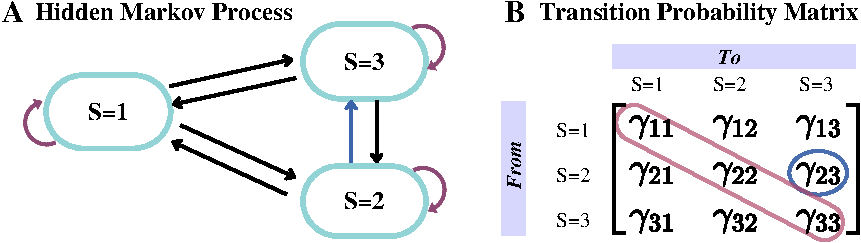
\includegraphics[width=0.8\textwidth]{graphics/time_hmm_s2.pdf}
\flushleft
\footnotesize
\justifying
Panel A: A visual representation of the Hidden Markov Process, where straight arrows represent transitions between states and curved arrows represent self-transitions. Panel B: The Transition Probability Matrix summarizing the Hidden Markov Process, where the diagonal entries are the probabilities of self-transitions and off-diagonal entries are the probabilities of transitioning between two different states. For example, $\gamma_{11}$ is the probability of remaining in the same state $S=1$ at the next time step of the process.
 \label{hmm_fig2}
\end{figure}

\subsection{The Multilevel Hidden Markov Model}
Following the work of \cite{altman_mixed_2007} we extend the \ac{hmm} to a multilevel framework by implementing subject-specific random effects. This extends the \ac{hmm} framework \linebreak to a hierarchical setting where subject-specific parameters can be estimated, allowing individual differences in underlying processes to be incorporated. In \ac{mhmm} assumptions introduced for \ac{hmm} and described with Equation \ref{ee1} and \ref{e2} remain, while the number of parameters extends by the number of added random effects. Below, we describe the \ac{mhmm} parameters' derivation process. 

The subject-specific transition probabilities $\gamma_{nij}$ are modelled from a set of multinomial logits $\alpha_{nij}$ using: 
\begin{equation}\label{e3}
 \gamma_{nij}= \frac{exp(\alpha_{nij})}{1+\sum_{s=2}^{m} exp(\alpha_{nis})}
\end{equation}
where
\begin{equation}
\label{e4}
\alpha_{nij}=\bar{\alpha}_{ij}+\epsilon_{nij} \end{equation}
for each individual ${n\in \left ( 1,..., N\right )}$, and each ${i, j\in \left \{ 1,..., m \right \}}$, where $N$ is the total number of individuals and $m$ is defined as before, with $\bar{\alpha}_{ij}$ being the (group-level) average logit for transitioning from state $i$ to state $j$, and $\epsilon_{nij}$ denotes the subject-specific deviation from the average. The individual-level random effects $\epsilon_{nij}$ follow a multivariate normal distribution with zero mean vector of length $m(m-1)$ and covariance matrix $\Sigma_{[\alpha]}$.
To ensure the identifiability of the $\Gamma$'s estimates, the numerator of the multinomial logit in Equation \ref{e3} is fixed at $1$ for $j=1$, making the transitions to the first state reference category in each row of $\Gamma$. Throughout the remainder of this text, we refer to the group-level average logit $\bar{\alpha}_{ij}$ as the TPM group-level fixed effects, and the (diagonal) variance components $\sigma^{2}_{[\alpha]ij}$ from the covariance matrix $\Sigma_{[\alpha]}$ the TPM individual-level random effects.
The subject-specific emission probability denoted as $Pr(y_{nt}|S_t=i)$ and interpreted as in Equation \ref{e2} is inferred from the Normal distribution (as in Equation \ref{e5}) with subject-specific mean $\mu_{ni}$ defined as:
\begin{equation}\label{e6}
 \mu_{ni}=\bar{\mu}_{i}+u_{ni}
\end{equation}
where for each individual ${n\in \left ( 1,..., N\right)}$ and state $i\in \left \{ 1,..., m \right \}$, $\bar{\mu}_{i}$ is the (group-level) mean of the dependent variable for each state and $u_{ni}$ denotes the individual-level deviation from the group-level mean. The $u_{ni}$ follow a normal distribution with mean 0 and variance $\sigma^{2}_{[\mu]i}$ fixed for all $i$. The variance $\sigma^{2}_{i}$ (refer to Equation \ref{e5}) of subject-specific emission distribution fixed across individuals. Throughout the remainder of this text, we refer to the group-level dependent variable mean $\bar{\mu}_{i}$ and variance $\sigma^{2}_{i}$ as the emission distribution group-level fixed effects, and the variance vectors $\sigma^{2}_{[\mu]i}$ the emission distribution individual-level random effects.

\subsection{Multilevel Explicit-Duration Hidden Markov Model}

The Explicit-Duration Hidden Markov Model  \citep[EDHMM;][]{freguson1980variable} is a more general form of the \ac{hmm}, where the memoryless assumption of the dwell times, specific to the \ac{hmm}, is relaxed. The self-transitions dictating the dwell times of each state in \ac{hmm} are redundant in \ac{edhmm}. Instead, the dwell time is explicitly derived from the set of state-specific dwell time distributions (see Figure \ref{edhmm_fig} for a detailed example of the \ac{edhmm}). Since transitions between states in the \ac{edhmm} follow the Hidden Markov Process and only self-transitions are replaced with dwell time distributions, the model assumes that latent states follow the Hidden Semi-Markov Process (see Figures \ref{edhmm_fig2}A and \ref{edhmm_fig2}B for an illustrative example of the assumption). 
\begin{figure}[]
\caption{\\The structure of the Explicit-duration Hidden Markov Model} 
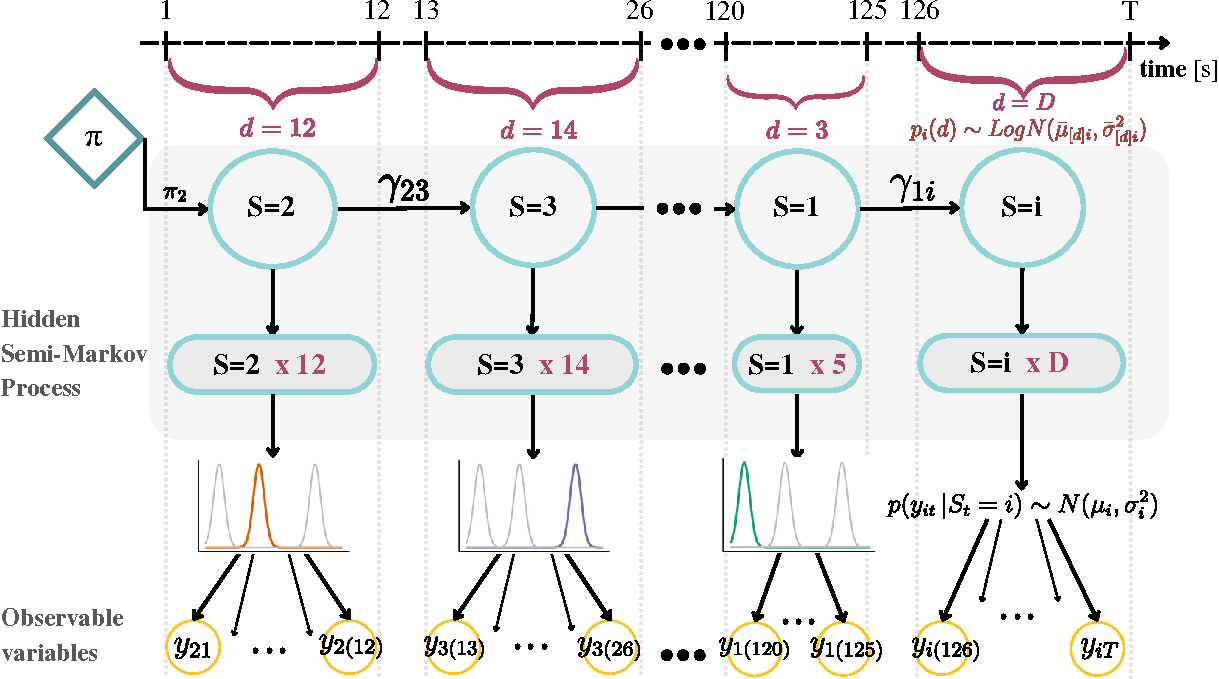
\includegraphics[width=\textwidth]{graphics/time_ed2.pdf}
 \flushleft
 \footnotesize
 \justifying
 The structure of the Explicit-duration Hidden Markov Model is based on three hidden states model and one normally distributed dependent variable. The model can be defined by four sets of parameters: 1) the vector $\pi$ of initial probabilities where $\pi_2$ is a probability of $S=2$ to be the initial state, 2) the TPM $\Gamma$ with $\gamma_{ij}$ for all $i\neq j$, and $\gamma_{23}$ represent the probability of switching from $S=2$ to $S=3$, 3) the state-specific dwell time distributions, in this case, the log-normal, and 4) the state-dependent emission distributions of observed events $y_t$ generated from hidden states. The dwell-times $d$ are drawn from the log-normal distributions each time the system transition to a new state $S$ i.e. when at time point $t=13$ latent state switch from S=2 to S=3 the dwell-time d=14 is drawn from the log-normal distribution with parameters specific to $S=3$. 
\label{edhmm_fig}
\end{figure}

\begin{figure}
\centering
\caption{\\The Hidden Semi-Markov Process for the three-state }
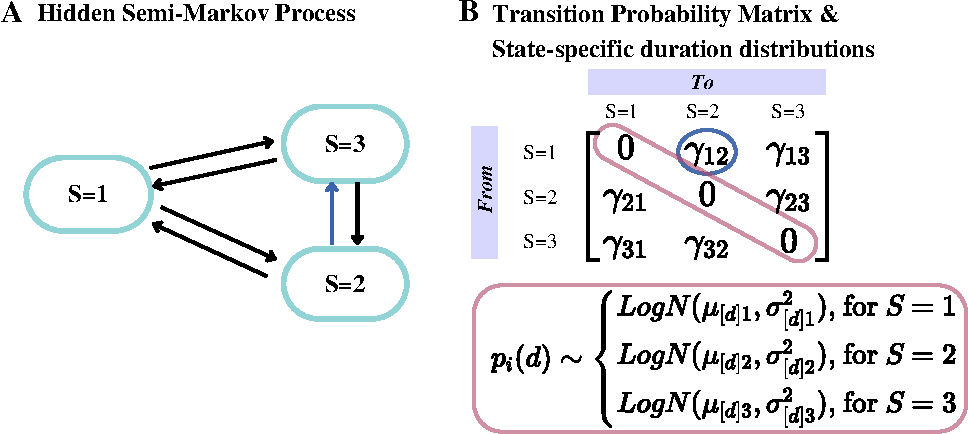
\includegraphics[width=0.85\textwidth]{graphics/time_edhmm_s2.pdf}
\flushleft
\footnotesize
\justifying
Panel A: A visual representation of the Semi-Markov Process. The straight arrows represent transitions between states. In comparison to Figure \ref{hmm_fig2}A self-transitions (curved arrows Figure \ref{hmm_fig2}A) are redundant in EDHMM. Panel B: The Transition Probability Matrix of the process, where the diagonal entries equal to $0$ and off-diagonal entries are the probabilities of transitioning between two different states e.g., $\gamma_{13}$ is the probability of transitioning from state $S=1$ to state $S=2$ at the next time step of the process. Instead of diagonal entries in the TPM, the set of dwell-time probabilities is assumed by the EHMM (outlined in red, below TPM).
 \label{edhmm_fig2}
\end{figure}
\newpage
In the Semi-Markov Process, the transition probabilities depend on a previous state ${S_{t}=i}$, as in \ac{hmm}(and \ac{mhmm}), and its duration $d_{S_{t}=i}$:
\begin{equation}
 Pr(S_t=i \rightarrow S_{t+1}=j)=Pr(S_{t+1}=j|S_{t}=i,d_{S_{t}=i})=\gamma_{ij} \\\text{, for } i\neq j,
\end{equation}
where the $d_{S_{t}=i}$ is a random integer from the range ${\left [ 1, d_{max} \right ]}$, and $d_{max}$ is the maximum allowable state duration.

The subject-specific dwell time probability for \ac{medhmm} is defined as:
\begin{equation}
\label{eq5}
 p_{i}(d_n)=Pr(S_{t+1:t+d_n]}=i|S_{[t+1:}=i)\text{, with} \sum^{d_{max}}_{d_n=1}p_{i}(d_n)=1,
\end{equation}
i.e. the probability that a state $i$ starts exactly at time ${t + 1}$ and ends at exactly ${t + d_n}$. The probabilities for all possible subject-specific state durations $d_n$ must sum up to $1$ for each state $i$. Note that we focused on the right-censored formulation here \citep{Guédon_2007}, which means that in the last visited state, the duration is estimated to be no longer than $M-t$, where $t$ is the current time point of observation and $M$ is the total length of the observation sequence.

In order to make the likelihood computation feasible, we obtain the probability of state-dependent duration $d_n$ only for whole units of time $t$. It implies that the state-specific dwell time distribution $p_i(d_n)$ is discrete. However, in case one assumes a parametric distribution, the $p_{i}(d_n)$ can be defined by any imposed distribution. To ease the burden of likelihood computation while maintaining flexibility in dwell time estimation in the current study, we consider $p_{i}(d_n)$ log-normally distributed. In addition, the distribution was most feasible to use in a Bayesian context that we intend to apply. \newpage That said, we can represent the $p_{i}(d_{n})$ as:
\begin{equation}
 p_{i}(d_{n})\sim LogNormal\left ( \mu_{[d]ni}, \bar{\sigma}^2_{[d]i} \right )
\end{equation}
with 
\begin{equation}
\mu_{[d]ni}=\bar{\mu}_{[d]i}+q_{ni}
\end{equation}
where, for each individual ${n\in \left ( 1,..., N\right )}$ and state ${i\in \left \{ 1,..., m \right \}}$, $\mu_{[d]ni}$ is the subject-specific log-mean and $\bar{\sigma}^2_{[d]i}$ the group-level log-variance. The subject-specific deviations from the group-level log-mean $\bar{\mu}_{[d]i}$ are denoted as $q_{ni}$ and normally distributed with mean zero and variance $\sigma^{2}_{[d]i}$, fixed across all individuals $n$. Furthermore, $\mu_{[d]i}$ and $\mu_{[d]ni}$ are means of the log-transformed durations, and $\exp{(\mu_{[d]i})}$, as well as, $\exp{(\mu_{[d]ni})}$ are medians of the untransformed durations. That said, for more intuitive descriptions, we will use the medians of the dwell time distributions ($\exp{(\mu_{[d]i})}$ and $\exp{(\mu_{n[d]i})}$) to describe the expected state durations and from this point onwards we will refer to it as mean/expected state duration or dwell time.

Since self-transitions are not estimated in the \ac{medhmm}, the $\Gamma$ is defined such that the diagonal entries $\gamma_{nij}$ for ${i=j}$ and ${i,j\in(1,2,...,m)}$ are equal to $0$. The off-diagonal entries of $\Gamma$ are derived similarly to the \ac{mhmm} presented in Section $2.2$ with Equation \ref{e3} adjusted such that transitions to the first state with non-zero probability, are the reference categories in each row of the TPM. Upon transitioning to a state $i$, in \ac{medhmm} a sequence of observations ${y_t, y_{t+1},...,y_{t+d_n}}$ of length $d_n$ is emitted from the emission distribution (refer to Equation \ref{e2}-3 and Equation \ref{e6}).

Note that in both \ac{mhmm} and \ac{medhmm} models, the number of states $m$ must be determined a priori by the researcher. Choosing the number of hidden states without a theoretical justification becomes a model selection problem for which standard criteria can be applied (e.g., Akaike information criteria (AIC), the Bayesian information criterion (BIC) etc.). For a detailed discussion on the issue, we refer the reader to \cite{de_haan_rietdijk_use_2017}. 

%\subsubsection*{The choice of the dwell time distribution}
%There are many options for dwell time distribution that researchers have successfully implemented. The two main determinants of appropriate dwell time are the subject of analysis and the compatibility of the proposed distribution with estimation algorithms. The Poisson duration distribution was used to model duration in speech recognition by \citep{1168477}. The Inverse gamma duration distribution has been used by \cite{Nagaraja_1996} to model patients’ staying time in the hospital. The Coxian distribution has been applied by \cite{1595592} to the task of recognizing activities of daily living in a smart house environment. In chapter 5 of \cite{Emm_Th} Log-normal duration distribution has been assumed to capture the movement stages of mice behaviours. In the study, we chose the Log-normal distribution as the distribution of the state-dependent duration probabilities, since it is most feasible to use in a Bayesian context that we intend to apply. 

% \begin{equation}
% p_i(d)\sim LogNormal(\mu_{[d]i},\sigma^2_{[d]i})
% \end{equation}
% where $\mu_{[d]i}$, denotes the logmean (i.e., the mean of the log-transformed durations) and $\exp{(\mu_{[d]i})}$ is the median of the (untransformed) durations, and $\sigma^2_{[d]i}$ denotes the variance in the log-transformed durations. As the median duration
% is more intuitive to interpret than the mean of the log-transformed durations, we will
% often use the median duration, denoted by $\exp{(\mu_{[d]i})}$, to describe the state durations.

% All in all, the \ac{edhmm} can be defined by four sets of parameters: the vector $\pi$ of initial probabilities $\pi_i$, TPM $\Gamma$, the set of parameters of state-dependent dwell time distributions and the set of parameters of the state-dependent probability distribution of observed events $y_t$.






% \subsection{Hidden Markov Model and Explicit-duration Hidden Markov Model in multilevel framework} 

% Traditionally, \ac{hmm}s, as well as \ac{edhmm}s, were applied to a time-series data sequence such as speech or written text (eg. \cite{Rabiner_1989} [\ac{hmm}], \cite{freguson1980variable} [\ac{edhmm}]). Behavioural and social data, however, are frequently collected as a series of observations (\ac{ild}) from multiple individuals. The collected data often resembles a hierarchical structure (add citation), where time-series observations are nested within individuals. Considering the extra complexity of the data, a few fitting data approaches have been taken to exploit the information effectively. (now I will present the 3 approaches and express a favour towards the last one. I'm editing the part now). One way is to fit models on pooled data, not considering possible correlations within the observations that are due to the hierarchical structure of the data. In that way, we obtain average results across the investigated group. We ignore the individual homogeneity of observation and heterogeneity between participants but we get average estimates of the sample parameters. On the other hand, for each participant, we can fit a separate hidden Markov Model (Mixture Hidden Markov Model). The method has been used in many publications (e.g ... \cite{visser_mixture_2022}). The Mixture Hidden Markov Model allow for the investigation of trends in sequences characteristic of the subject. However, it is highly computationally intensive and doesn't give us a chance to refer the individual patient's dynamics to the group-level estimates. Note that multiple hidden Markov models might result in best models that vary in terms of the number of states for example. It is not correct since the aim of a study is usually to compare participants on a given fixed condition. Finally, one can apply the \ac{hmm} or \ac{hsmm} in a Multilevel framework (short \ac{mhmm} and \ac{mhsmm}). \ac{mhmm}s and \ac{mhsmm}s that take into account both the homogeneity of observations between subjects and heterogeneity of individuals, while treating it all as the same system. That way, we are able to model the complex data system under one model. In the multilevel framework, we account for individual variability by introducing individual random effects, which can be seen as individual deviations to fixed group-level estimates of parameters of the \ac{hmm} and \ac{edhmm}.


%Note that $\mu_{[d]i}$ and $\mu_{n[d]i}$ are means of the log-transformed durations, and $\exp{(\mu_{[d]i})}$ and $\exp{(\mu_{n[d]i})}$ are medians of the (untransformed) durations. That said, for more intuitive descriptions, we will often use the medians of durations ($\exp{(\mu_{[d]i})}$ and $\exp{(\mu_{n[d]i})}$) to describe the state durations.


% A potential issue that may arise during Bayesian estimation of the \ac{mhmm} or \ac{edhmm} is what has been referred to as label switching \citep{Celeux_Hurn_Robert_2000}.The most common way to prevent label switching has been defining appropriate starting values and having well-defined and distinct (not overlapping) state distributions. 

% The Bayesian approach eliminates the need for numerical integration and enables interval estimation as a direct product of the estimation routine. Simulation-based methods, such as the Markov chain Monte Carlo approach [20] including the Metropolis-Hasting algorithm [21, 22] and the Gibbs sampler [23], make the Bayesian approach relatively easily adaptable to complex latent variable models that are more difficult to fit in the frequentist setting.

% There is no straightforward criterion for model fit or model selection that can be used to choose the number of latent states when that number is not known a priori. Researchers working in the frequentist framework often use the Akaike Information Criterion (AIC; Akaike, 1974) or Bayesian Information Criterion (BIC; Schwarz, 1978) for model comparison and for choosing the number of latent states. Other methods used has been DIC Bayes Factor 
% In the Bayesian framework, the exact Bayes factor for model comparison is difficult to implement, and both exact and approximate Bayes Factors (such as the BIC approximation, cf. Kass & Raftery, 1995) yield results that depend on a specific prior distribution (Frühwirth-Schnatter, 2006). Another commonly used criterion is the Deviance Information Criterion (DIC; Spiegelhalter, Best, Carlin, & Van Der Linde, 2002), but there is no consensus on the right way to define the DIC for multilevel models (Celeux, Forbes, Robert, & Titterington, 2006).
% A potential issue that may arise during Bayesian estimation of the \ac{mhmm} or \ac{edhmm} is what has been referred to as label switching (\cite{Celeux_Hurn_Robert_2000}. The problem is caused due to the fact that the likelihood of a Bayesian multilevel model could be invariant to permutations of the values, “labels”, of the discrete latent variable. This may lead to uninterpretable results Hence we should always make an effort to prevent it from happening. The most common way to prevent label switching has been defining appropriate starting values and having well-defined and distinct (not overlapping) state distributions which we made sure to implement on our study.